%---------------------------------------------------------------------------
% System deployment description.
%
%---------------------------------------------------------------------------


\section{System Deployment}
\label{sec:deployments}

The simplest possible deployment of SemSimMon if depicted in Figure~\ref{fig:depl_simple}. As we can see, in this scenario all monitoring components are running on a single machine. User has started a monitored application (either a single Java application, or even a MainSM) either on own PC or on some other remote host (these 2 cases are similar from SemSimMon\rq{}s point of view), then used the Monitoring Hub built-in to the GUI component. Transport proxies communicate with the monitored applications using a loopback or a real network interface, and all communication between Monitoring Hub and GUI uses the process\rq{}s memory.

\begin{figure}[h]
   \centering
   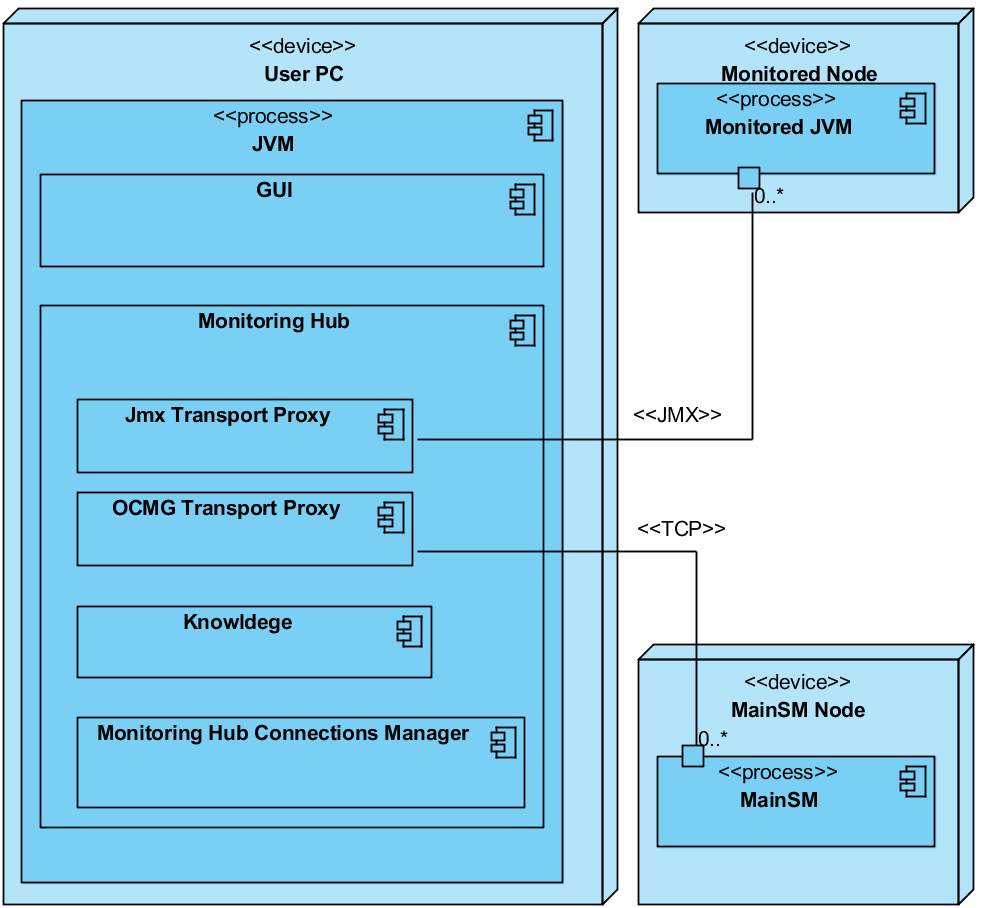
\includegraphics[width=0.6\textwidth]{simplest_deployment}
   \caption{Simplest deployment diagram}
   \label{fig:depl_simple}
 \end{figure}
 
In contrast to the above scenario, Figure~\ref{fig:depl_complex} depicts the most complex deployment model. In this case, user has started the GUI application using own PC, but the Monitoring Hub (one or more) runs in a separate JVM (either in the same, local PC or any other remote host). Connection between these components is established as RMI over TCP/IP. Additionally the Monitoring Hub communicates with one or more (again, optionally remote) applications of interest. This deployment is used, when the user launches the GUI application, the monitored applications and chooses to use a remote Monitoring Hub Application while adding resources. It allows the most flexible measurements and allows using the makes the system capable of measuring large scale applications.

\begin{figure}[h]
   \centering
   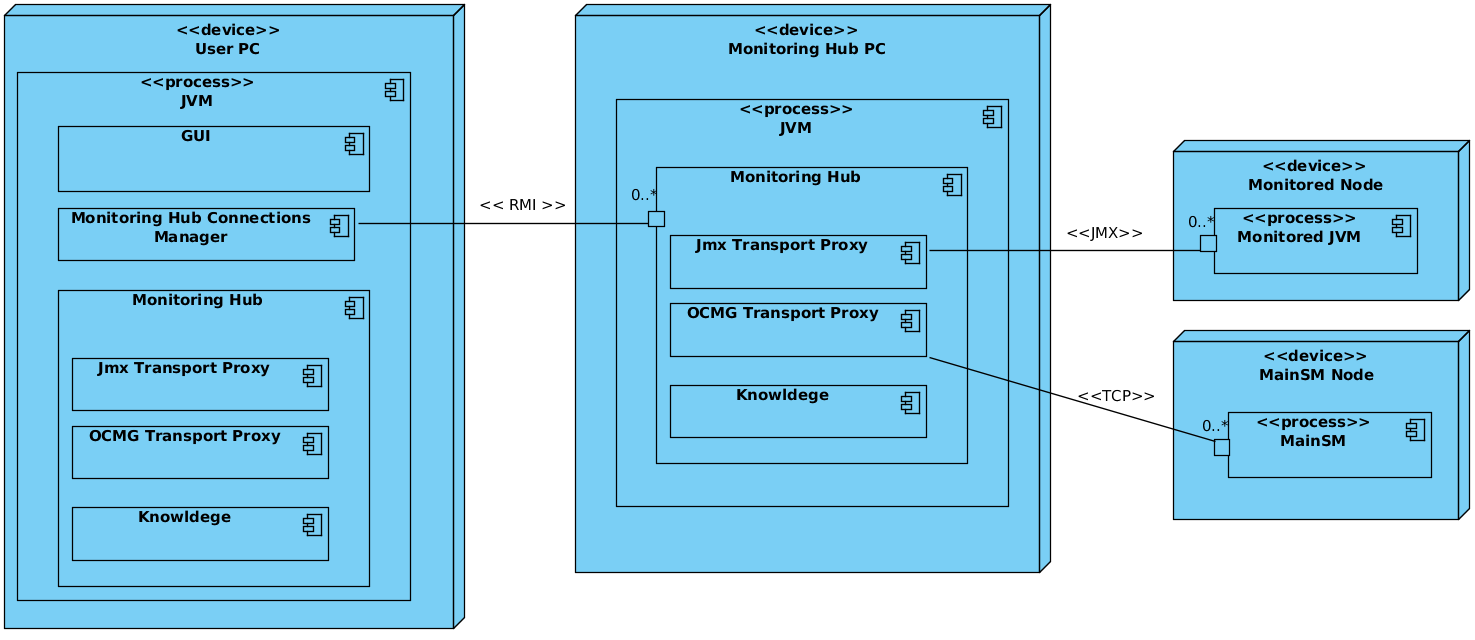
\includegraphics[width=1\textwidth]{distributed_deployment}
   \caption{Distributed deployment diagram}
   \label{fig:depl_complex}
 \end{figure}
